\documentclass[a4paper,12pt]{article}
\usepackage{mathtools}
\usepackage{graphicx}
\usepackage{subcaption}
\usepackage{booktabs}
\usepackage{amsthm}
\usepackage{amsfonts}
\usepackage{hyperref}
\usepackage{tcolorbox}
\usepackage{listings}
\usepackage{xcolor}
\usepackage{markdown}

\definecolor{codegreen}{rgb}{0,0.6,0}
\definecolor{codegray}{rgb}{0.5,0.5,0.5}
\definecolor{codepurple}{rgb}{0.58,0,0.82}
\definecolor{backcolour}{rgb}{0.95,0.95,0.92}

\lstdefinestyle{mystyle}{
    backgroundcolor=\color{backcolour},   
    commentstyle=\color{codegreen},
    keywordstyle=\color{magenta},
    numberstyle=\tiny\color{codegray},
    stringstyle=\color{codepurple},
    basicstyle=\ttfamily\footnotesize,
    breakatwhitespace=false,         
    breaklines=true,                 
    captionpos=b,                    
    keepspaces=true,                 
    numbers=left,                    
    numbersep=5pt,                  
    showspaces=false,                
    showstringspaces=false,
    showtabs=false,                  
    tabsize=2
}
%\usepackage{lineno}
\newcommand{\norm}[1]{\left\lVert#1\right\rVert}

\setlength{\parindent}{0em}
\setlength{\parskip}{0.5em}
\begin{document}
\title{COVID-19 Forecasting}
\date{}
%\large 
%\author{Che-Chia Chang}
%\IEEEtitleabstractindextext{%
%    \begin{abstract}
%        Abstract-In this 
%    \end{abstract}
%}
\author{Che-Chia Chang}
%\address{Department of Applied Mathematics, National Chiao Tung University}
%\begin{abstract}

%\end{abstract}
\maketitle
%\IEEEdisplaynontitleabstractindextext

\section{Introduction}
We would like to predict the future confirmed and deaths results of the COVID-19. If forecasting can be done, we would be able to be prepared of what would happened, also it would be useful when a similar pandemic happens, we can use our experience to examine the data in such case.
\section{Preprocessing}
\subsection{The Data}
We will use the dataset from JHU CSSE COVID-19 Data which can be downloaded from \href{https://github.com/CSSEGISandData/COVID-19}{https://github.com/CSSEGISandData/COVID-19}. We will use the \href{https://github.com/CSSEGISandData/COVID-19/blob/master/csse_covid_19_data/csse_covid_19_time_series/time_series_covid19_confirmed_global.csv}{confirmed} and \href{https://github.com/CSSEGISandData/COVID-19/blob/master/csse_covid_19_data/csse_covid_19_time_series/time_series_covid19_deaths_global.csv}{deaths} global datasets on their page. The files are csv files with format

\begin{tabular}{llrrrrr}
        \toprule
        Province/State & Country/Region &       Lat &       Long &  1/22/20 &  1/23/20 &  1/24/20 \\
        \midrule
                   NaN &    Afghanistan &  33.93911 &  67.709953 &        0 &        0 &        0 \\
                   NaN &        Albania &  41.15330 &  20.168300 &        0 &        0 &        0 \\
                   NaN &        Algeria &  28.03390 &   1.659600 &        0 &        0 &        0 \\
                   NaN &        Andorra &  42.50630 &   1.521800 &        0 &        0 &        0 \\
                   NaN &         Angola & -11.20270 &  17.873900 &        0 &        0 &        0 \\
        \bottomrule
\end{tabular}

here only the first few row and columns are listed. It consists the State, Region, the geographic location (latitude and longitude) and the confirmed/deaths each day starting from 2020/1/22. We collect the confirmed and deaths of each country into a array for later usage.
\subsection{Data Windowing}
We use the confirmed and death collected explained in previous section to train the model. We generate the training data by splitting the data in to windows, a example of a window can be given as following figure.
\begin{center}
    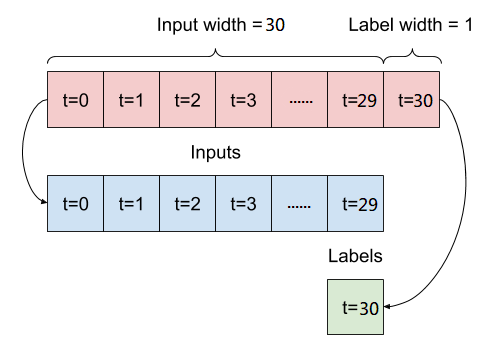
\includegraphics{split_window.png}
\end{center}
In this example, we split out dataset so that we wish to come up with a model that predict 1 day of confirmed/deaths given 30 days of confirmed/deaths datas. Later we will demonstrate different results with different data windowing.

\subsection{Normalization}
We normalize the given data by each window. Given an confirmed or deaths input window \(\mathbf{x}\), which should be a array. If we use the windowing example as previous subsection, we get an array of $30$ elements of confiremd/deaths people that day. We calculate the mean \(\mu(\mathbf{x})\) and variance \(\sigma(\mathbf{x})\), then the actual input data \(\hat{\mathbf{x}}\) will be given by 
\[\hat{\mathbf{x}}_i = \frac{\mathbf{x}_i - \mu(\mathbf{x})}{\sigma(\mathbf{x})} \quad \text{ if } \sigma(\mathbf{x})\neq 0, \]
and 
\[\hat{\mathbf{x}}_i = \mathbf{x}_i - \mu(\mathbf{x}) \quad \text{ if } \sigma(\mathbf{x})= 0\]
for each \(i\), where \(\mathbf{x}_i\) and \(\hat{\mathbf{x}}_i\) are elements of \(\mathbf{x}\) and \(\hat{\mathbf{x}}\) respectively.

For the output data \(\mathbf{y}\), we will apply the mean and variance of the input window to get the actual output data \(\hat{\mathbf{y}}\), that is 
\[\hat{\mathbf{y}}_i = \frac{\mathbf{y}_i - \mu(\mathbf{x})}{\sigma(\mathbf{x})} \quad \text{ if } \sigma(\mathbf{x})\neq 0, \]
and 
\[\hat{\mathbf{y}}_i = \mathbf{y}_i - \mu(\mathbf{x}) \quad \text{ if } \sigma(\mathbf{x})= 0\]
for each \(i\), where \(\mathbf{y}_i\) and \(\hat{\mathbf{y}}_i\) are elements of \(\mathbf{y}\) and \(\hat{\mathbf{y}}\) respectively.
%![Alt](./split_window.png) 
\section{Models}
The models will be implemented by using following libraries in Python: \href{https://xgboost.readthedocs.io/en/latest/python/python_intro.html}{XGBoost}, \href{https://scikit-learn.org/}{Scikit-learn}, and \href{https://www.tensorflow.org}{TensorFlow}.
\subsection{XGBoost}
First model we will try the infamous gradient boosting based library XGBoost. We omit the details here, but one can have a quick look at XGBoost's \href{https://xgboost.readthedocs.io/en/latest/tutorials/model.html}{docs} to have a quick look at XGBoost. Note that when predicting more days, since XGBoost only supports single output regression default, we will use scikit-learn's \href{https://scikit-learn.org/stable/modules/generated/sklearn.multioutput.MultiOutputRegressor.html}{MultiOutputRegressor} as a wrapper, which simply fits one regressor per target. 
\subsection{Linear Regression}
We use standard linear regression model, which will be implemented by the scikit-learn library. We also use MultiOutputRegressor when predicting multiple days. 
\subsection{Dense Neural Network}
We will use a simple dense neural network which is consists of two hidden layers with 64 neurons, while the layers are passed with activation function relu. The implementation will be using TensorFlow.
\section{Results}
The following results comparison of different models where the windowing and the training/testing set splitting are different, we will specify the details. Currently (2020/12/22), the time series data consists of 335 days of data. A score of each model will be calculated using the following rules.
Let $\hat{Y} = \{\hat{\mathbf{y}_i}\}$ be the predicted values, and let $Y =\{ \mathbf{y}_i\}$ be the corresponding true values, the predict score is defined as  
\[\text{score}  = 1 - \frac{\sum_i (\hat{\mathbf{y}_i} - \mathbf{y}_i)^2}{\sum_i (\mathbf{y}_i - \mu(Y))^2  },\]
where $\mu(Y)$ is the mean of $Y$. This gives us a glance at how well the model is as $1$ giving the best score, but one should not only look at this score to determine if a model's useful. In the following, we will also demonstrate the forecasting results of a given country, we will calculate the maximum error where both the dataset and the prediction has a value.
\subsection{Multiple countries as training sets}
First results comes where we use US, Spain, Belgium, China, France, Germany, United Kingdom, Italy data as training sets, but also keeping the last 150 days of data out of the windowing. All the other data window pairs will be collected as the testing set. 
\subsubsection{1 day prediction}
Here we will predict $1$ day by $30$ days. We'll show the output of our program, which shows the training/testing score of each model and the maximum error and prediction figure of the model. 
\begin{tcolorbox}
Data length:	 335

\begin{tabular}{lrrr}
\toprule
 Training score   &   xgboost &   linear regression &   dense network \\
\midrule
 Confirmed        &  0.999968 &            0.813265 &        0.886461 \\
 Deaths           &  0.999985 &            0.566096 &        0.575712 \\
\bottomrule
\end{tabular}


\begin{tabular}{lrrr}
\toprule
 Testing score   &    xgboost &   linear regression &   dense network \\
\midrule
 Confirmed       & -0.788356  &            0.12582  &         0.31407 \\
 Deaths          &  0.0378059 &            0.163331 &         0.17573 \\
\bottomrule
\end{tabular}
\end{tcolorbox}
\begin{tcolorbox}
    Japan

    \begin{tabular}{lrrr}
    \toprule
     Max error   &   xgboost &   linear regression &   dense network \\
    \midrule
     Confirmed   &  1574.32  &           3076.88   &       3030.49   \\
     Deaths      &   599.835 &             41.3703 &         42.4389 \\
    \bottomrule
    \end{tabular}
        
    \begin{center}
        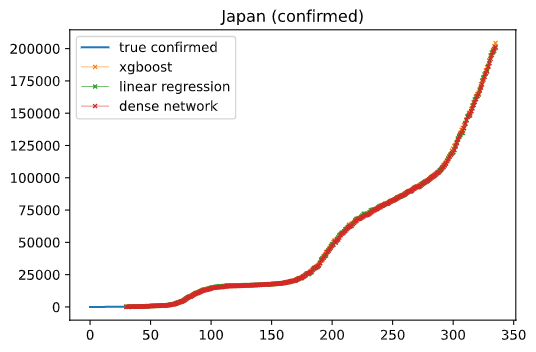
\includegraphics[width=1\textwidth]{Japan_1-1.png}
        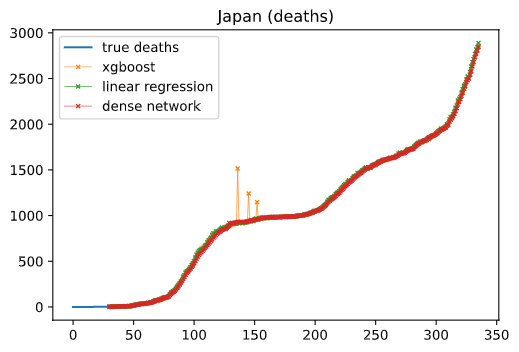
\includegraphics[width=\textwidth]{Japan_1-2.png}
    \end{center}

\end{tcolorbox}
We will omit other output of other countries. We see the dense network is giving the best score in testing, while XGBoost has the best score in training. In the output we given, XGBoost is giving the least maximum error in confirmed, but it gives the largest error in deaths.

\subsubsection{10 days prediction}
Here we'll show predictions of 10 days by inputting 30 days. To draw the figure of prediction, since there will be overlapping days of predictions, we simply skip 10 days to prevent overlapping and combine the figure.
\begin{tcolorbox}
    Data length:	 335

    \begin{tabular}{lrrr}
    \toprule
    Training score   &   xgboost &   linear regression &   dense network \\
    \midrule
    Confirmed        &  0.99999  &            0.527157 &        0.591767 \\
    Deaths           &  0.999992 &            0.595707 &        0.666162 \\
    \bottomrule
    \end{tabular}


    \begin{tabular}{lrrr}
    \toprule
    Testing score   &    xgboost &   linear regression &   dense network \\
    \midrule
    Confirmed       & -41.751    &           -13.6738  &       -1.96249  \\
    Deaths          &  -0.522273 &            -1.43025 &       -0.457888 \\
    \bottomrule
    \end{tabular}
\end{tcolorbox}
\begin{tcolorbox}
    Japan
    
    \begin{tabular}{lrrr}
    \toprule
    Max error   &   xgboost &   linear regression &   dense network \\
    \midrule
    Confirmed   &  12425.2  &          242591     &       52186.7   \\
    Deaths      &   1158.32 &             571.676 &         389.853 \\
    \bottomrule
    \end{tabular}
    \begin{center}
        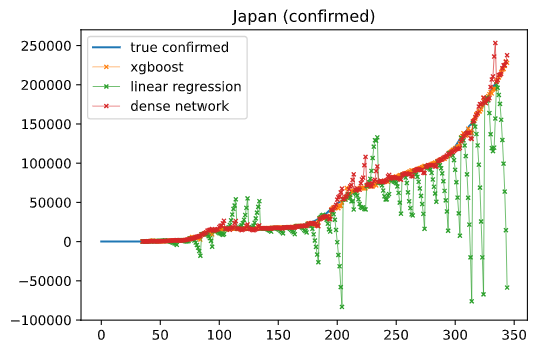
\includegraphics[width=\textwidth]{Japan_2-1.png}
        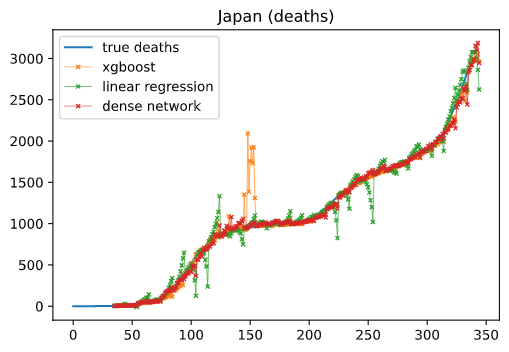
\includegraphics[width=\textwidth]{Japan_2-2.png}
    \end{center}
\end{tcolorbox}
In here linear regression definitely gives the worst results. In overall dense network has better score, but in some cases, as the Japan's confirmed we shown, XGBoost perform much better.
\subsubsection{30 days prediction}
Here we use 30 days to predict 30 days.
\begin{tcolorbox}
    Data length:	 335

    \begin{tabular}{lrrr}
    \toprule
    Training score   &   xgboost &   linear regression &   dense network \\
    \midrule
    Confirmed        &  0.999997 &            0.467218 &        0.256903 \\
    Deaths           &  0.999997 &            0.490763 &        0.295669 \\
    \bottomrule
    \end{tabular}


    \begin{tabular}{lrrr}
    \toprule
    Testing score   &   xgboost &   linear regression &   dense network \\
    \midrule
    Confirmed       &  -21.9279 &            -11.9818 &        -1.95719 \\
    Deaths          &  -47.6586 &            -70.5059 &       -33.2122  \\
    \bottomrule
    \end{tabular}

\end{tcolorbox}
\begin{tcolorbox}
    Japan

    \begin{tabular}{lrrr}
    \toprule
    Max error   &   xgboost &   linear regression &   dense network \\
    \midrule
    Confirmed   &  52348    &         1.99932e+07 &     5.86749e+06 \\
    Deaths      &   6619.66 &     56423.7         &  3741.35        \\
    \bottomrule
    \end{tabular}
    \begin{center}
        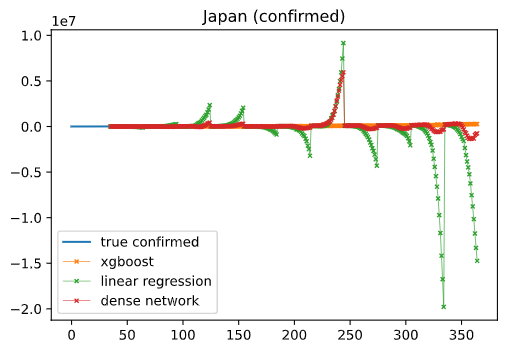
\includegraphics[width=\textwidth]{Japan_3-1.png}
        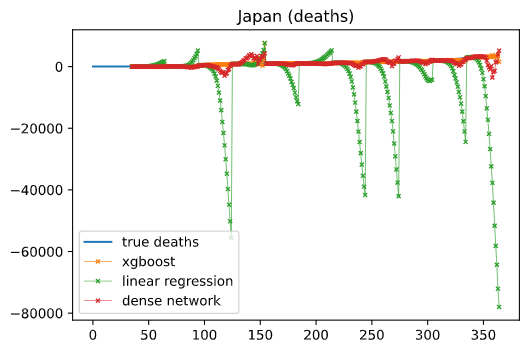
\includegraphics[width=\textwidth]{Japan_3-2.png}
    \end{center}
\end{tcolorbox}
The results are similar to the 10 days one with linear regression being weaker.
\subsection{Taiwan as training set}
It is interesting to try Taiwan's dataset as the training set, since Taiwan has very few infected and deaths, so we may want to see in this case how the model performs. Interestingly, we notice that the multi-day prediction of deaths performs even better in this case.
\subsubsection{1 day prediction}
\begin{tcolorbox}
    Data length:	 335

    \begin{tabular}{lrrr}
    \toprule
    Training score   &   xgboost &   linear regression &   dense network \\
    \midrule
    Confirmed        &  0.999999 &            0.872291 &        0.766207 \\
    Deaths           &  1        &            0.862836 &        0.845123 \\
    \bottomrule
    \end{tabular}


    \begin{tabular}{lrrr}
    \toprule
    Testing score   &   xgboost &   linear regression &   dense network \\
    \midrule
    Confirmed       &  0.373952 &           0.359536  &        0.369799 \\
    Deaths          &  0.123399 &           0.0616844 &        0.169387 \\
    \bottomrule
    \end{tabular}

\end{tcolorbox}
\begin{tcolorbox}
    Japan
    \begin{tabular}{lrrr}
    \toprule
    Max error   &   xgboost &   linear regression &   dense network \\
    \midrule
    Confirmed   &  2505.31  &           2187.56   &       4456.09   \\
    Deaths      &   126.151 &             50.9315 &         63.4678 \\
    \bottomrule
    \end{tabular}

    \begin{center}
        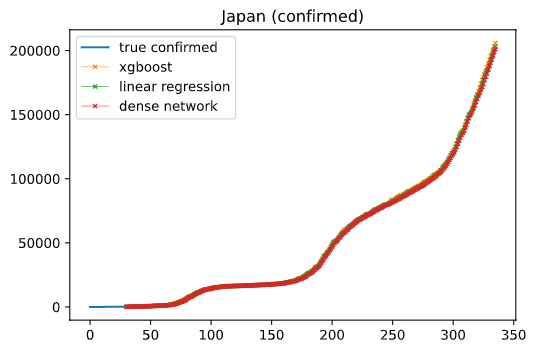
\includegraphics[width=\textwidth]{Japan_4-1.png}
        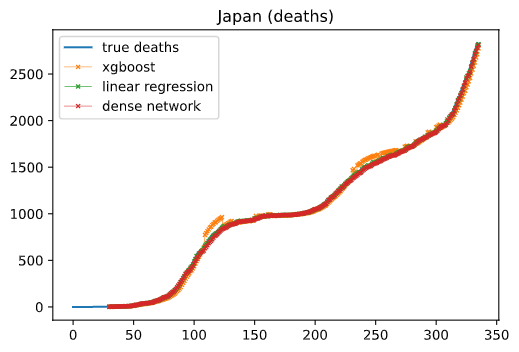
\includegraphics[width=\textwidth]{Japan_4-2.png}
    \end{center}
\end{tcolorbox}
\subsubsection{10 days prediciton}
\begin{tcolorbox}
    Data length:	 335
    
    \begin{tabular}{lrrr}
    \toprule
     Training score   &   xgboost &   linear regression &   dense network \\
    \midrule
     Confirmed        &         1 &            0.74128  &        0.38569  \\
     Deaths           &         1 &            0.750351 &        0.748695 \\
    \bottomrule
    \end{tabular}
    
    
    \begin{tabular}{lrrr}
    \toprule
     Testing score   &   xgboost &   linear regression &   dense network \\
    \midrule
     Confirmed       & 0.0715908 &           -0.126634 &       0.0118868 \\
     Deaths          & 0.029451  &           -3.15018  &       0.0911274 \\
    \bottomrule
    \end{tabular}
    
\end{tcolorbox}
\begin{tcolorbox}
    Japan

    \begin{tabular}{lrrr}
    \toprule
     Max error   &   xgboost &   linear regression &   dense network \\
    \midrule
     Confirmed   & 14870.1   &            20440.4  &       11261.9   \\
     Deaths      &   439.813 &              220.61 &         348.709 \\
    \bottomrule
    \end{tabular}

    \begin{center}
        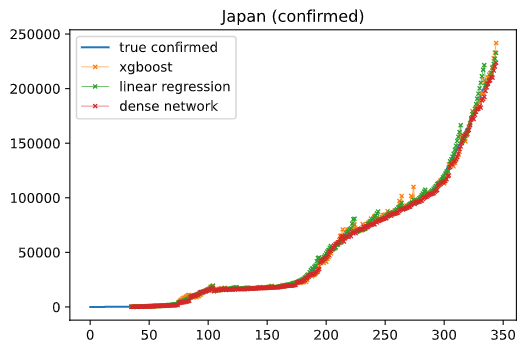
\includegraphics[width=\textwidth]{Japan_5-1.png}
        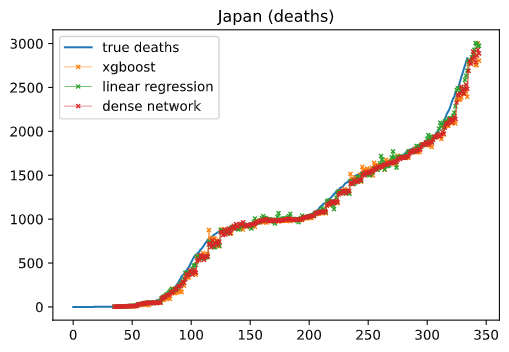
\includegraphics[width=\textwidth]{Japan_5-2.png}
    \end{center}
\end{tcolorbox}
\subsubsection{30 days prediction}
\begin{tcolorbox}
    Data length:	 335

    \begin{tabular}{lrrr}
    \toprule
     Training score   &   xgboost &   linear regression &   dense network \\
    \midrule
     Confirmed        &         1 &            0.592588 &        0.244347 \\
     Deaths           &         1 &            0.731003 &        0.378217 \\
    \bottomrule
    \end{tabular}
    
    
    \begin{tabular}{lrrr}
    \toprule
     Testing score   &   xgboost &   linear regression &   dense network \\
    \midrule
     Confirmed       & 0.0247015 &           0.0661764 &    -0.00124943  \\
     Deaths          & 0.0231771 &          -0.0743319 &     0.000458915 \\
    \bottomrule
    \end{tabular}
    

\end{tcolorbox}
\begin{tcolorbox}
    Japan

    \begin{tabular}{lrrr}
    \toprule
    Max error   &   xgboost &   linear regression &   dense network \\
    \midrule
    Confirmed   &    326330 &          140927     &       68258     \\
    Deaths      &       530 &             343.506 &         608.476 \\
    \bottomrule
    \end{tabular}


    \begin{center}
        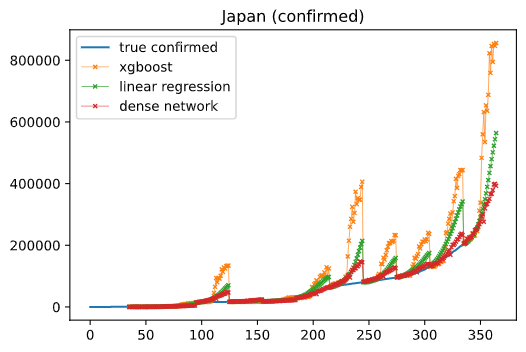
\includegraphics[width=\textwidth]{Japan_6-1.png}
        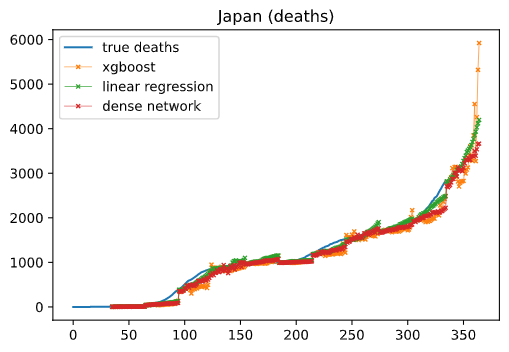
\includegraphics[width=\textwidth]{Japan_6-2.png}
    \end{center}
\end{tcolorbox}

\section{The program}
\subsection{How to run}
Here we demonstrate how to run our program in UNIX environment. A similar instruction can be found at \href{https://github.com/twMisc/COVID-19-Forecasting-Python}{https://github.com/twMisc/COVID-19-Forecasting-Python}. Suppose one has python3, pip, git installed. First download the dataset and our program. 
\lstset{style=mystyle}
\begin{lstlisting}[language=bash]
$ git clone https://github.com/CSSEGISandData/COVID-19/
$ git clone https://github.com/twMisc/COVID-19-Forecasting-Python
$ cd COVID-19-Forecasting-Python
\end{lstlisting}
Install the required packages in Python.
\begin{lstlisting}[language=bash]
$ pip install xgboost numpy tensorflow scikit-learn tabulate matplotlib plotly pandas
\end{lstlisting}
Alternatively, install the requirements using requirements.txt if you encountered into some trouble.
\begin{lstlisting}[language=bash]
$ pip install -r requirements.txt    
\end{lstlisting}
Then modify the file \texttt{forecasting\_setup.py} as required
\begin{lstlisting}[language=Python]
observe_days = 30
predict_days = 1
keepdays = 150
training_countries = ['US','Spain']
\end{lstlisting}
\begin{itemize}
    \item \texttt{observe\_days}: input data length
    \item \texttt{predict\_days}: output data length
    \item \texttt{keepdays}: the length of data to NOT use in training
    \item \texttt{training\_countries}: the countries to be used in training, can be found in \texttt{country\_list.txt}
\end{itemize}
Run \texttt{forecasting\_run.py} in console to see the results if you want a quick glance.
\begin{lstlisting}[language=bash]
$ python forecasting_run.py
\end{lstlisting}

\subsection{Run in Visual Studio Code interactive window
}
To use this, you must have a Python environment where you have installed the \href{https://pypi.org/project/jupyter/}{Jupyter Package}. You should also install the  \href{https://marketplace.visualstudio.com/items?itemName=ms-python.python}{Python extension} in VScode. Check out VScode's \href{https://code.visualstudio.com/docs/python/jupyter-support-py}{doc} if you want to learn more.

Open \texttt{forecasting\_run.py} in VScode, which also includes some explanation.

\subsection{Run in Jupyter Notebook}
If you have \href{https://jupyter.org/install.html}{Jupyter Notebook or JupyterLab} installed, you can use them as well.

Open \texttt{forecasting\_run.ipynb} in JupyterLab or the classic Jupyter Notebook.

\subsection{Run it in Python interpreter}
You can also use the function yourself in your python console. After setting up \texttt{forecasting\_setup.py}, in python, run something like
\begin{lstlisting}[language=Python]
>>> from forecasting_multi import print_and_draw
>>> print_and_draw('Japan') 
\end{lstlisting}
Replace Japan with any country in \texttt{country\_list.txt}. Note that two html plot files \texttt{forecasting\_confirmed.html} and \texttt{forecasting\_deaths.html} generated by Plotly should also be available after running 
\begin{lstlisting}[language=Python]
print_and_draw(country_name).
\end{lstlisting}
where \texttt{country\_name} is your input.

\section{Conclusion}
In our experiment, while linear regression may be useful if we want to predict only 1 day, the fails to predict well if more days are required. The XGBoost and dense neural network will be more useful in such case. In general we suggest using XGBoost or the dense network when predicting multiple days. The XGBoost model may still be improved since we do not have any correlation for the predict days, if we define some custom objective function the results may be improved.

Also, the testing results may vary depend on the training set chosen. If we choose the training countries more carefully, results may still be improved.
\end{document}
